\documentclass[11pt]{article}
\usepackage[T1]{fontenc}
\usepackage[utf8]{inputenc}
\usepackage{lmodern}
\input{glyphtounicode}
\pdfgentounicode=1
\usepackage{amsmath,amssymb,amsthm,geometry,booktabs,graphicx,hyperref}
\geometry{margin=1in}
\emergencystretch=1em
\hypersetup{colorlinks=true,linkcolor=blue,citecolor=blue,urlcolor=blue,
  pdftitle={A rich 5-ary word with critical exponent E*(u_9)},
  pdfauthor={Qianghao Wu},
  pdfkeywords={rich words, palindromes, critical exponent, repetition threshold, bispecial factors, morphic words}}
\newtheorem{theorem}{Theorem}
\newtheorem{lemma}[theorem]{Lemma}
\newtheorem{proposition}[theorem]{Proposition}
\newtheorem{conjecture}[theorem]{Conjecture}
\theoremstyle{remark}
\newtheorem{remark}[theorem]{Remark}
\newcommand{\w}[1]{\textup{\texttt{#1}}}
\newcommand{\file}[1]{\texttt{\detokenize{#1}}}
\newcommand{\Bext}{\operatorname{Bext}}
\newcommand{\Pext}{\operatorname{Pext}}
\newcommand{\RT}{\operatorname{RT}}
\title{A rich word over five letters with critical exponent $E^*(u_9)$,\\ and the bound $\RT(C_5)\le E^*(u_9)\approx 2.0592854$}
\author{Qianghao Wu}
\date{November 26, 2026}
\begin{document}
\maketitle

\begin{abstract}
A finite word of length $n$ is rich if it has $n+1$ distinct palindromic factors,
counting the empty word. The repetition threshold $\RT(C_d)$ is the infimum of the
critical exponents of the infinite rich words over $d$ letters. Let $u_d$ be the fixed
point of $\varphi_d\colon i\mapsto 0(i+1)$ for $i<d-1$, $d-1\mapsto 0(d-1)(d-1)$.
Dvořáková and Pelantová conjectured that $\RT(C_d)=E^*(u_{2d-1})$, where $E^*$ is the
asymptotic critical exponent. The conjecture is known for $d=2,3,4$. Dvořáková, Mol and
Pelantová (2026) named a first step for $d\ge5$: find a morphism
$\pi\colon\Sigma_{2d-1}^*\to\Sigma_d^*$ such that $\pi(u_{2d-1})$ is rich and has critical
exponent $E^*(u_{2d-1})$. We give such a morphism for $d=5$. The letter images have
lengths $2,3,1,2,4,6,11,19,36$. So $\RT(C_5)\le E^*(u_9)=1+1/(3-\Lambda)\approx
2.0592854490$, where $\Lambda$ is the root of $t^5-2t^4-1$ in $(2,3)$. The proof
reduces the critical exponent to bispecial factors and their return words, by a theorem
of Dolce, Dvořáková and Pelantová. We describe all bispecial factors of $\pi(u_9)$ from
seven exceptional bispecial factors of $u_9$ and sixteen infinite chains. A program compares each ratio
with $1/(3-\Lambda)$ in exact arithmetic, and bounds the tail of each chain with a
closed form. Two programs written separately confirm the result, and a brute-force search
on long prefixes agrees with it. The lower bound $\RT(C_5)\ge E^*(u_9)$ remains open.
This work has not yet been reviewed by experts. The computations, the proofs and the
text were produced by AI models (from Anthropic and OpenAI), working under the author's
direction.
\end{abstract}

\noindent Status: Computer-assisted. This work has not yet been reviewed by experts.
There is no proof-assistant formalization.

\section{Introduction}

A finite word $w$ of length $n$ has at most $n+1$ distinct palindromic factors, counting
the empty word. It is \emph{rich} if it has exactly $n+1$. An infinite word is rich if
all of its factors are rich. Rich words were introduced by Droubay, Justin and
Pirillo~\cite{djp}. For a nonempty word $v$ and a rational $e\ge1$, the word $v^e$ is the
prefix of length $e|v|$ of $vvv\cdots$. The \emph{critical exponent} of an infinite word
$x$ is
\[
E(x)=\sup\{e\in\mathbb Q : v^e \text{ is a factor of } x \text{ for a nonempty word } v\},
\]
and the \emph{asymptotic critical exponent} $E^*(x)$ is the $\limsup_{n\to\infty}$ of the
same set with $|v|=n$. Always $E^*(x)\le E(x)$. With $\Sigma_d=\{0,1,\dots,d-1\}$ and
$C_d$ the class of infinite rich words over $\Sigma_d$, the source paper~\cite{dmp}
defines
\[
\RT(C_d)=\inf\{E(x) : x \text{ is an infinite rich word over } \Sigma_d\}.
\]

\paragraph{The words $u_d$.} Let $\varphi_d(i)=0(i+1)$ for $i\in\{0,\dots,d-2\}$ and
$\varphi_d(d-1)=0(d-1)(d-1)$, and let $u_d$ be the fixed point of $\varphi_d$. Dvořáková,
Klouda and Pelantová~\cite{dkp} showed that $u_d$ is rich and that
$E^*(u_d)=1+1/(3-\Lambda_d)$, with $\Lambda_d$ the spectral radius of the incidence matrix
of $\varphi_d$. They also showed that the asymptotic repetition threshold of rich words is
$2$ for every alphabet size. Dvořáková and Pelantová~\cite{dp-limit} proved that
$\RT(C_d)\to2$ as $d\to\infty$, by morphic images of $u_{2d+1}$ over $d+2^d$ letters, and
they stated the conjecture below.

\paragraph{Known values.} Currie, Mol and Rampersad~\cite{cmr} proved
$\RT(C_2)=E^*(u_3)\approx2.70710678$. Currie, Mol and Peltomäki~\cite{cmp} proved
$\RT(C_3)=E^*(u_5)\approx2.25876324$; the morphic form of their extremal word is due to
Dvořáková and Pelantová~\cite{dp-sym}. Dvořáková, Mol and Pelantová~\cite{dmp} proved a
structure theorem for $d=4$ and obtained $\RT(C_4)=E^*(u_7)\approx2.1197196907$
\cite[Corollary~1.6]{dmp}.

\begin{conjecture}[{\cite[Conjecture~1.1]{dmp}, from~\cite{dp-limit}}]\label{conj}
For every integer $d\ge2$, we have $\RT(C_d)=E^*(u_{2d-1})$.
\end{conjecture}

Section~8 of~\cite{dmp} lists open questions. Its first item reads:
\begin{quote}
``A first step towards proving Conjecture 1.1 for every $d\ge5$ would be to find a
projection $\pi=\pi_d:\Sigma^*_{2d-1}\to\Sigma^*_d$ such that $\pi(u_{2d-1})$ is rich and
$E(\pi(u_{2d-1}))=E^*(u_{2d-1})$. This would prove the inequality
$\RT(C_d)\le E^*(u_{2d-1})$.''
\end{quote}
In~\cite{dmp} a \emph{projection} is a morphism from the larger alphabet to the smaller
one; letter images can be long (Table~1 of~\cite{dmp}). We do this step for $d=5$, the
first open case.

\begin{theorem}\label{thm:main}
Let $\pi\colon\Sigma_9^*\to\Sigma_5^*$ be the morphism of Table~\ref{tab:pi}, and let
$z=\pi(u_9)$. Then $z$ is rich and
\[
E(z)=E^*(u_9)=1+\frac1{3-\Lambda}\approx 2.0592854490,
\]
where $\Lambda\approx2.0559673967$ is the root of $t^5-2t^4-1$ in $(2,3)$. Hence
$\RT(C_5)\le E^*(u_9)$.
\end{theorem}

\begin{table}[ht]
\centering
\begin{tabular}{@{}rlr@{}}
\toprule
$i$ & $\pi(i)$ & $|\pi(i)|$\\
\midrule
0 & \w{01} & 2\\
1 & \w{011} & 3\\
2 & \w{0} & 1\\
3 & \w{02} & 2\\
4 & \w{0232} & 4\\
5 & \w{023432} & 6\\
6 & \w{02343223432} & 11\\
7 & \w{0234344343343443432} & 19\\
8 & \w{023434434334344343234344343343443432} & 36\\
\bottomrule
\end{tabular}
\caption{The projection $\pi$ (candidate A in the programs). Each $\pi(i)$ is $0$
followed by a palindrome without $0$.}
\label{tab:pi}
\end{table}

\paragraph{What is new.} The searches recorded with this result (citations of~\cite{dmp}
and~\cite{dp-limit}, arXiv, GitHub, Zenodo and other sources, last checked on
November 26, 2026) found no projection for $d=5$ and no upper bound on $\RT(C_5)$ at
$E^*(u_9)$. The public code of~\cite{dmp} covers $d=3$ and $d=4$ only. The new content is
the morphism of Table~\ref{tab:pi} and the computer-assisted proof of
Theorem~\ref{thm:main}. We do not prove the lower bound $\RT(C_5)\ge E^*(u_9)$. In the
cases $d\le4$ that bound came from a structure theorem~\cite{cmr,cmp,dmp}.

\paragraph{The status of the proof.} The proof cites three published results
(Section~\ref{sec:cited}) and uses a computer for a finite list of exact checks and for
an eigenvalue estimate in 60-digit floating point. Section~\ref{sec:limits} lists all
assumptions.

\section{Cited results}\label{sec:cited}

For a factor $w$ of an infinite word $x$, let $\Bext(w)=\{(a,b): awb \text{ is a factor
of } x\}$, with $a,b$ letters. The word $w$ is \emph{bispecial} if it has at least two
left and two right extensions. Its \emph{bilateral order} is
$b(w)=\#\Bext(w)-\#\{a\}-\#\{b\}+1$, and for a palindrome $w$,
$\Pext(w)=\{(a,a)\in\Bext(w)\}$. If $j<\ell$ are consecutive occurrences of $w$ in
$x=x_0x_1\cdots$, then $x_j\cdots x_{\ell-1}$ is a \emph{return word} to $w$.

\begin{itemize}
\item[(T1)] \cite[Theorem~3]{ddp}, quoted as Theorem~7.2 in~\cite{dmp}. If $x$ is
uniformly recurrent and aperiodic, then
$E(x)=1+\sup\{|w|/|r| : w \text{ bispecial in } x,\ r \text{ a return word to } w\}$.
\item[(T2)] \cite[Theorem~4]{dp-limit}. If the language of $x$ is closed under reversal,
then $x$ is rich if and only if every bispecial factor $w$ satisfies $b(w)=0$ when $w$ is
not a palindrome, and $b(w)=\#\Pext(w)-1$ when $w$ is a palindrome.
\item[(T3)] \cite{dkp}, as listed in~\cite[Section~2]{dp-limit}: the language of $u_d$
is closed under reversal, and $E^*(u_d)=1+1/(3-\Lambda_d)$, with $\Lambda_d$ the root in
$(2,3)$ of $t^{d-1}(t-2)^2-1$. For $d=9$ we have
$t^8(t-2)^2-1=(t^5-2t^4-1)(t-1)(t^4-t^3-t^2-t-1)$, so $\Lambda_9=\Lambda$.
\end{itemize}

The source~\cite[Proposition~7.4]{dmp} (from~\cite[Proposition~19]{dp-limit}) gives a
shorter richness test for morphisms of class $P_{\mathrm{ret}}$. Our $\pi$ is of this
class with marker $0$. We check its hypothesis, but the proof below uses (T2) on every
bispecial factor, so it does not depend on that proposition.

\section{\texorpdfstring{Bispecial factors of $u_9$ and of $z$}{Bispecial factors of u9 and of z}}\label{sec:proof}

Write $u=u_9$, $\varphi=\varphi_9$, $M$ for the incidence matrix of $\varphi$ ($9\times9$),
$h_i=|\pi(i)|$, and $\vec w$ for the Parikh vector of a word $w$, so that
$|\pi(w)|=h\cdot\vec w$. Put $P_5(t)=t^5-2t^4-1$, $Q_4(t)=t^4-t^3-t^2-t-1$ and
$q=1/(3-\Lambda)\approx1.0592854490$. The characteristic polynomial of $M$ is
$P_5Q_4$, with nine distinct roots. The four roots of $P_5$ other than $\Lambda$ have
modulus at most $0.8886$. The roots of $Q_4$ include one real root
$\beta\approx1.9276$.

\begin{lemma}[blocks]\label{lem:blocks}
The letter $0$ occurs in $u$ exactly at the first letter of each block $\varphi(u_j)$.
So the letters $1,\dots,7$ are always preceded and followed by $0$, and $88$ is always
preceded and followed by $0$.
\end{lemma}

\begin{lemma}[desubstitution]\label{lem:desub}
The bispecial factors of $u$ of length at most $1$ are $\varepsilon$, $0$ and $8$. Every
bispecial factor $w$ of $u$ with $|w|\ge2$ has the form $w=s\,\varphi(w')\,0\,t$ with
$s,t\in\{\varepsilon,8\}$ and $w'$ a shorter bispecial factor of $u$, its
\emph{parent}. The extensions of $w$ follow from $\Bext(w')$ by an explicit rule:
$(a,b)\in\Bext(w')$ gives the pair (last letter of $\varphi(a)$, second letter of
$\varphi(b)$) when $s=t=\varepsilon$, and similar rules for $s=8$ or $t=8$, which
admit only $a\in\{7,8\}$ or $b\in\{7,8\}$.
\end{lemma}

Both lemmas follow from the fact that each $\varphi(c)$ starts with $0$ and has no other
$0$. So the bispecial factors of $u$ form a tree with roots $\varepsilon$ and $8$. A node
is a \emph{$2\times2$ node} if it has exactly two left and two right extensions, and a
\emph{multi node} otherwise.

\begin{lemma}[chains]\label{lem:chain}
A $2\times2$ node $w'$ has exactly one bispecial child, and this child is again a
$2\times2$ node. Each occurrence of $w'$ gives an occurrence of the child, so the return
words of the child have Parikh vectors $M\vec r$, for the return words $r$ of $w'$.
\end{lemma}

The program expands the tree from the roots. The expansion stops with $7$ multi nodes, of
lengths $0,1,3,7,15,31,63$, and $16$ \emph{seeds}: the root $8$, which is a $2\times2$ node, and the $2\times2$ nodes
whose parent is a multi node, of lengths $1,2,2,4,4,8,8,16,16,32,32,64,64,127,128,128$. By
Lemmas~\ref{lem:desub} and~\ref{lem:chain}, every bispecial factor of $u$ is a multi node
or lies on the infinite chain $w_0,w_1,w_2,\dots$ of one seed $w_0$.

The images $\pi(i)=0x_i$, with $x_i$ a palindrome without $0$, put a $0$ at the start of
each block. So a factor $v$ of $z$ without $0$ lies inside some $x_c$, and a factor $v$
with a $0$ has a unique form $v=x\,\pi(w)\,0\,y$, with $x$ a suffix of some $x_a$, $y$ a
prefix of some $x_b$ and $w$ a factor of $u$. If $v$ is bispecial, then $w$ is bispecial
in $u$. For a $2\times2$ node $w$ with $\Bext$ letters $a,a'$ on the left and $b,b'$ on
the right, exactly one bispecial factor of $z$ has this $w$:
\[
v(w)=\operatorname{lcs}(\pi(a),\pi(a'))\,\pi(w)\,\operatorname{lcp}(\pi(b)0,\pi(b')0),
\]
and the return words of $v(w)$ have lengths $h\cdot\vec r$ for the return words $r$ of
$w$. So the bispecial factors of $z$ are: the empty word, $15$ nonempty factors without
$0$, $51$ factors from multi nodes, and the factors $v(w_n)$ on the $16$ chains.

\begin{lemma}[exact comparison]\label{lem:exact}
For integers $a,b\ge1$: $a/b<q$ if and only if $P_5(3-b/a)<0$.
\end{lemma}

\begin{proof}
$a/b<q$ is equivalent to $3-b/a<\Lambda$. For $s\le2$ we have $P_5(s)=s^4(s-2)-1<0$, and
$P_5$ is increasing on $(8/5,\infty)$ with the single root $\Lambda$ there.
\end{proof}

\paragraph{Return words of the seeds.} The program builds the prefix $\varphi^{21}(0)$ of
$u$, of length $2\,310\,194$. The $17$ two-letter factors of $u$ all occur in
$\varphi^9(0)$, so this prefix contains every factor of $u$ of length at most $4153$.
For each seed $w$, let $W$ be the length of the longest window of the prefix that
contains no occurrence of $w$. If $W+2\le4153$, then every factor of $u$ of length $W+1$
contains $w$, so every return word $r$ satisfies $|r|+|w|-2\le W$, and $rw$ occurs in
the prefix. So the gaps between consecutive occurrences in the prefix give all return
words. Each of the $16$ seeds passes this test and has exactly $9$ return words. This
certificate replaces the cited fact that every factor of $u_9$ has $9$ return words.

\paragraph{Chains.} Along each chain, the type of the node (its $\Bext$ and the letters
$s,t$) is periodic with period $8$ from $n=0$, for all $16$ seeds. For a seed, a return
word $r$, and $n\ge0$, put $a_n=|v(w_n)|$ and $b_n=h\cdot M^n\vec r$. We need
$a_n/b_n<q$ for all $n$.

\begin{lemma}[tail]\label{lem:tail}
Write $n=8N+i$ with $0\le i<8$. Then $D_n:=q\,b_n-a_n=h\cdot M^nX+c_i$, where $X$ is a
vector with entries in $\mathbb Q(\Lambda)$ and the $c_i$ are rational numbers, all
computed from the seed and $r$. Expanding in eigenvectors,
$h\cdot M^nX=\sum_\mu\kappa_\mu\mu^n$. The coefficients $\kappa_\mu$ vanish for the four
roots of $Q_4$, because $h$ is orthogonal to their right eigenvectors. Hence
\[
D_n\ \ge\ \kappa_\Lambda\Lambda^n+c_i-\varepsilon\rho^n,\qquad
\varepsilon=\sum_{\mu\ne\Lambda,\ P_5(\mu)=0}|\kappa_\mu|,\quad \rho\le0.8886.
\]
\end{lemma}

The orthogonality $h\cdot v_\mu=0$ for the roots of $Q_4$ is the length condition of
\cite[Proposition~17]{dp-limit}. With
$v_t=(t^7(t-2),\dots,t(t-2),t-2,1)$ it becomes four linear equations:
$h_5=h_0+h_4$, $h_6=h_1-h_4+2h_5$, $h_7=h_2-h_4+2h_6$, $h_8=h_3-h_4+2h_7$. The program
checks it exactly, as a remainder modulo $Q_4$.

\section{Proof of Theorem~\ref{thm:main}}\label{sec:main}

The word $z$ is uniformly recurrent, as a morphic image of the fixed point of a primitive
morphism. It is aperiodic: the cut of $z$ at its letters $0$ recovers $u$, and the letter
frequencies of $u$ are irrational because $P_5$ is irreducible. The language of $z$ is
closed under reversal, because the reversal of $\pi(w)0$ is $\pi(\overline w)0$ and the
language of $u$ is closed under reversal (T3).

\emph{Richness.} The program checks the condition of (T2) on the empty word, on the $15$
bispecial factors without $0$, on the $51$ factors from multi nodes, and on the chain
factors $v(w_n)$ for $n\le60$. Along a chain the type and the palindrome property are
periodic from $n=0$, so $n\le60$ covers every case. By (T2), $z$ is rich.

\emph{Upper bound.} For the $51+15$ finite cases, the program finds the shortest return
word in a prefix of $z$ that provably contains it, and checks $|v|/|r|<q$ by
Lemma~\ref{lem:exact}. For the chains, it checks $a_n/b_n<q$ exactly for $n\le60$. For
$n>60$ it uses Lemma~\ref{lem:tail}. It decides exactly, in $\mathbb Q[t]/(P_5)$, whether
$\kappa_\Lambda=0$. In $142$ of the $144$ pairs (seed, return word), $\kappa_\Lambda>0$,
with smallest value $2.14$, so $D_n\to\infty$. In the other $2$ pairs,
$\kappa_\Lambda=0$ and $\min_ic_i=2/5$, exactly. The largest $\varepsilon$ in these two
pairs is $0.5454$, and $\varepsilon\rho^n<2/5$ for $n\ge3$. In all cases $D_n>0$ for
$n>60$. So every ratio is below $q$, and $E(z)\le1+q$ by (T1).

\emph{Lower bound.} For the pair on the chain of the seed $w_0=8$ with $\kappa_\Lambda=0$,
$D_n$ stays bounded while $b_n\to\infty$. So $a_n/b_n\to q$ and $E(z)\ge1+q$ by (T1).

So $E(z)=1+q=E^*(u_9)$ by (T3). The word $z$ is an infinite rich word over $\Sigma_5$
(it uses all five letters), so $\RT(C_5)\le E(z)$. \qed

The two critical chains are those of the seed $w_0=8$ and of the seed of length $127$. The
largest ratio that the program meets is $a_{60}/b_{60}\approx1.0592854490$ on the chain
of the seed of length $127$, which is below $q$ by Lemma~\ref{lem:exact}.

\section{How the result was checked}\label{sec:checks}

The folder that accompanies this paper contains four programs. Its
\file{checks/README.md} gives the commands.

\begin{enumerate}
\item \file{checks/verify.py} does the proof of Section~\ref{sec:main} for a given
morphism. It uses exact rational and polynomial arithmetic (SymPy), and mpmath with
60 digits only for $\kappa_\mu$ ($\mu\ne\Lambda$), $\varepsilon$, $\rho$ and the sign of
a nonzero $\kappa_\Lambda$. It also compares the tree with the bispecial factors of $u$
of length at most $40$ found directly ($36$ factors). It ends with
\file{RESULT: ALL CHECKS PASSED}.
\item \file{checks/crosscheck.py} uses only $\varphi$, $\pi$ and prefixes of $z$. It
finds all bispecial factors of $z$ of length at most $60$ by brute force ($64$ factors)
and their shortest return words, and they equal the list that the theory predicts. It
also confirms all $149$ predicted bispecial factors of length at most $3000$.
\item \file{checks/independent_check.py} was written in the verification stage from the
definitions and the proof plan, before its author read \file{verify.py}. It finds by
brute force the $75$ bispecial factors of $u$ of length at most $300$ and the $146$
bispecial factors of $z$ of length at most $2000$, checks the condition of (T2) on all of
them, and checks $|v|/|r|<q$ for the $125$ of them with a certified shortest return word
(largest ratio $18/17$). It checks the chains exactly for $n\le1000$, with its own
closed form and tail bound. At $n=1000$ the term $\varepsilon\rho^n$ is below $10^{-50}$.
\item \file{checks/prefix_check.c} uses only the definitions. On the prefix of $z$ of
length $9\,727\,357$ (the image of $3\,000\,000$ letters of $u$), an eertree finds
$9\,727\,357$ distinct nonempty palindromes, so the prefix is rich. The largest exponent
of a repetition in this prefix, over all periods, is
$3684955/1789434\approx2.0592852265<E^*(u_9)$.
\end{enumerate}

Figure~\ref{fig:exp} shows the output of the last program: the largest exponent in each
band of periods rises towards $E^*(u_9)$ from below.

\begin{figure}[ht]
\centering
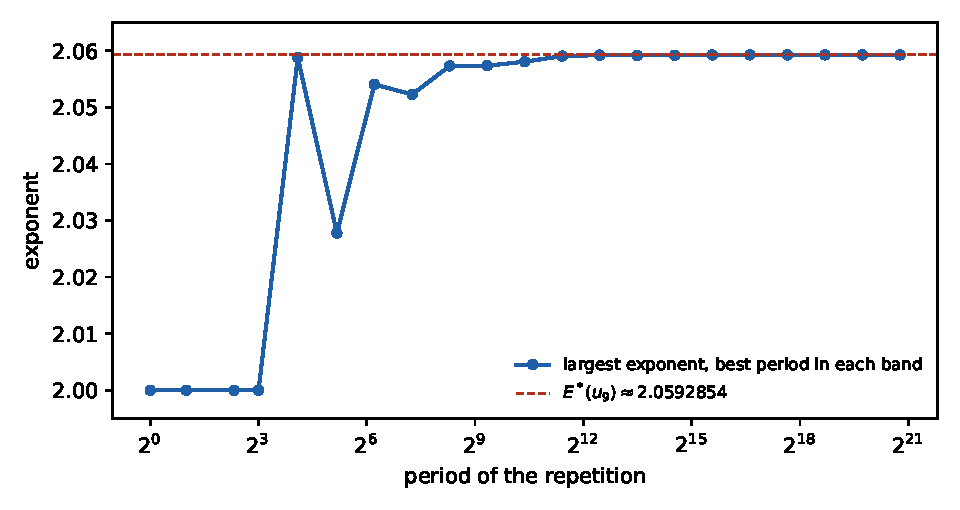
\includegraphics[width=0.8\textwidth]{exponents.pdf}
\caption{Largest exponent of a repetition in the first $9\,727\,357$ letters of $z$, for
periods in $[2^k,2^{k+1})$, $k=0,\dots,20$. The dashed line is $E^*(u_9)$.}
\label{fig:exp}
\end{figure}

\paragraph{Other projections.} Two more morphisms pass the same programs. Candidate B
differs from Table~\ref{tab:pi} only in $\pi(6)=\w{02343443432}$. Candidate C is
$0\mapsto\w{01}$, $1\mapsto\w{011}$, $2\mapsto\w{0}$, $3\mapsto\w{02}$,
$4\mapsto\w{022322}$, $5\mapsto\w{02234322}$, $6\mapsto\w{0223434434322}$,
$7\mapsto\w{022343443433434434322}$,
$8\mapsto\w{02234344343343443432343443433434434322}$. We did not check whether the
languages of the three words differ up to a permutation of the letters. So we do not
claim three distinct words.

\paragraph{How $\pi$ was found.} A depth-first search over morphisms of class
$P_{\mathrm{ret}}$ with marker $0$ and palindromic $x_i$ imposed the four linear equations
of Section~\ref{sec:proof}, and pruned by richness and by the largest exponent on prefixes
of $\pi(u_9)$. Three candidates survived on a prefix of $1200$ letters of $u_9$. The
search is not part of the proof.

\section{Limits}\label{sec:limits}

\begin{itemize}
\item The proof assumes (T1), (T2) and the two facts (T3) from the literature. We did not
re-prove them, and no program checks them.
\item The tail estimate of Lemma~\ref{lem:tail} uses 60-digit floating point for
$\kappa_\mu$ ($\mu\ne\Lambda$), $\varepsilon$ and $\rho$, not interval arithmetic. The
decision $\kappa_\Lambda=0$ is exact. The margins are large: every nonzero
$\kappa_\Lambda$ is at least $2.14$; where $\kappa_\Lambda=0$, $\min c_i=2/5$ against
$\varepsilon\rho^{60}<2\cdot10^{-3}$, and the exact check of \file{independent_check.py}
reaches $n=1000$, where $\varepsilon\rho^n<10^{-50}$.
\item The programs are not formally verified, and there is no Lean proof.
\item We do not prove $\RT(C_5)=E^*(u_9)$. The lower bound needs a structure theorem as
in~\cite[Section~6]{dmp}.
\end{itemize}

\begin{thebibliography}{9}

\bibitem{cmp}
J.~D.~Currie, L.~Mol and J.~Peltomäki,
\emph{The repetition threshold for ternary rich words},
Electron.\ J.\ Combin.\ \textbf{32}(2) (2025), \#P2.55,
\href{https://doi.org/10.37236/13499}{doi:10.37236/13499},
\href{https://arxiv.org/abs/2409.12068}{arXiv:2409.12068}.

\bibitem{cmr}
J.~D.~Currie, L.~Mol and N.~Rampersad,
\emph{The repetition threshold for binary rich words},
Discrete Math.\ Theor.\ Comput.\ Sci.\ \textbf{22}(1) (2020), article 6,
\href{https://doi.org/10.23638/DMTCS-22-1-6}{doi:10.23638/DMTCS-22-1-6}.

\bibitem{ddp}
F.~Dolce, L.~Dvořáková and E.~Pelantová,
\emph{On balanced sequences and their critical exponent},
Theoret.\ Comput.\ Sci.\ \textbf{939} (2023), 18--47,
\href{https://doi.org/10.1016/j.tcs.2022.10.014}{doi:10.1016/j.tcs.2022.10.014}.

\bibitem{djp}
X.~Droubay, J.~Justin and G.~Pirillo,
\emph{Episturmian words and some constructions of de Luca and Rauzy},
Theoret.\ Comput.\ Sci.\ \textbf{255} (2001), 539--553,
\href{https://doi.org/10.1016/S0304-3975(99)00320-5}{doi:10.1016/S0304-3975(99)00320-5}.

\bibitem{dkp}
L.~Dvořáková, K.~Klouda and E.~Pelantová,
\emph{The asymptotic repetition threshold of sequences rich in palindromes},
European J.\ Combin.\ \textbf{126} (2025), 104124,
\href{https://doi.org/10.1016/j.ejc.2025.104124}{doi:10.1016/j.ejc.2025.104124}.

\bibitem{dmp}
L.~Dvořáková, L.~Mol and E.~Pelantová,
\emph{An automated approach to structure theorems for minimally repetitive rich words},
\href{https://arxiv.org/abs/2611.13676}{arXiv:2611.13676v1}, November 10, 2026.

\bibitem{dp-sym}
L.~Dvořáková and E.~Pelantová,
\emph{Symmetries of rich sequences with minimum critical exponent},
in Combinatorics on Words (WORDS 2025), Lecture Notes in Comput.\ Sci.\ \textbf{15729},
Springer, 2025, 143--154,
\href{https://doi.org/10.1007/978-3-031-97548-6_11}{doi:10.1007/978-3-031-97548-6\_11},
\href{https://arxiv.org/abs/2501.15135}{arXiv:2501.15135}.

\bibitem{dp-limit}
L.~Dvořáková and E.~Pelantová,
\emph{The limit of repetition thresholds of rich sequences},
Electron.\ J.\ Combin.\ \textbf{33}(2) (2026), \#P2.15,
\href{https://doi.org/10.37236/14600}{doi:10.37236/14600},
\href{https://arxiv.org/abs/2509.06104}{arXiv:2509.06104}.

\end{thebibliography}
\end{document}
